\chapter{Evaluation and Findings}

\section{Testing the implementation} \label{sec:testing}
In order to keep tests fair, it is important to keep as much of the environment constant as possible between test iterations. Each iteration should have one variable that is changed so that the effects of this change can be easily observed and analysed. The following sections will outline the tests on how changing the volume of traffic that is sent between clients on a consumer network, effects the jitter with which the messages arrive.

The test is set up using the client hosted model where the clients are connected to the network on both an ethernet connection and WiFi. The host is connected to the router over ethernet cables that go through a switch. One client that will connect to the host is started on the same machine as the server; this client will be referred to as the ``localhost client''. Another client is connected directly to the router and it will be referred to as the ``ethernet client''. The last client that will connect to the host, is a laptop that is close to the router and connected over WiFi, this will be referred to as the ``WiFi client''.

Once the connection has been established, the server tick-rate can be configured. This will be the variable that will be changed and the effects of this will be observed at each stage of the experiment. To minimise any external factors that could effect this experiment, all tests were performed at night when the network is under least stress.

\subsection{Capturing and analysing the results}
When writing the GNAT library, one of the most important features was the custom wrapper for a logging library that would go on to be used extensively during the development and testing. This wrapper allows for a message to be written to a log file from anywhere in the program. The library code is written in such a way that any action that is done, is logged under different logging levels depending on the nature of the information. One piece of information that is logged whenever a message is received by a client, is the time that has elapsed since the last message that has been received. This information can then in turn be used to calculate the jitter of incoming messages and this is what is used to generate data in the following experiments.

A simple script was used to extract the values, on each log file (one for each client and therefore three for each test). The script would use RegEx to look for lines where the jitter information is logged and extract the number from the rest of the line. The output would be a file with 1 number per line which can then be fed into another program to generate graphs. The analysis of this data and some examples of the graphs produced in this way, can be found under the section \ref{sec:jitter_results}.

In order to compare how varied the numbers were from one another, each result set, was fed as input into a math function calculating the variance ($\sigma^2$) of the data. The analysis of this can be found in the section \ref{sec:variance_results}.

\newpage
\subsection{Jitter between WiFi and Ethernet connections} \label{sec:jitter_results}
The author's expectation for the results from this test were: more anomalous values would be present in WiFi packets rather than Ethernet packets due to the higher chance of packet loss and less reliable connection technology. The jitter in WiFi data is also expected to be more varied than a wired connection.
After harvesting and extracting the data from this experiment, over 5000 values were produced for each client and each test. Each number represents the time between two received messages arriving and so it is understandable that if a given packet takes longer then average to reach the client, a larger number will be produced however as a result when the next packet is received (after traveling for what can be assumed to be an average time), it is likely that the next value will be smaller than average. This nature, produces the zig-zag like shape that can be seen in the graphs where if there is a large spike in one direction, it is likely that the next data value, will then produce a large spike in the other direction. The graphs representing this data can be seen in figures \ref{fig:250ms_graph}, \ref{fig:64ms_graph} and \ref{fig:8ms_graph}. These graphs show the data for the WiFi client and the Ethernet client for 250ms, 64ms and 8ms server tick-rates respectively and each one has been limited to use the same amount of data to make the horisontal axis scale consistant.

For each dataset, the data turned out to be very similar; it can be seen that in general the data for the Ethernet client, arrived within 1 millisecond, however as expected, the data for the WiFi client appeared to be slightly more varied with most of the data arriving within 2 milliseconds of the average. Another anomaly that can be seen with the WiFi connection throughout each test, is that it is much more common for a ``random'' spike to occur. These spikes could occur due to several reasons. One example is that packet loss occurred causing the wait for the next packet to essentially double. This can be seen in several instances through one value having an abnormally large value but not followed by an abnormally small value directly after.

An effect that can be observed with the different tick-rates, is that it is much less common for abnormally large or small, anomalous data to be seen in WiFi connections as the tick-rate gets faster. As the tick-rate increases, each anomalous result (whether it is due to packet loss or suboptimal routing) is much less impactful if there is another packet arriving soon after. An exception to this rule however can be seen in the 8ms test. The packets in the data for the 8ms test appear much more varied in general more anomalous spikes can be seen in both WiFi and Ethernet data (despite this trend being more obvious in WiFi data). To show these anomalous spikes more clearly, the scale has been streatched to 2.5ms per horisontal line instead of 1ms like it is on the other graphs. Unfortunately, it is unclear why this exception occurs in this test when in every other test, the variance can be seen to be getting smaller.

\newpage
\begin{figure}[p]
  \centering
  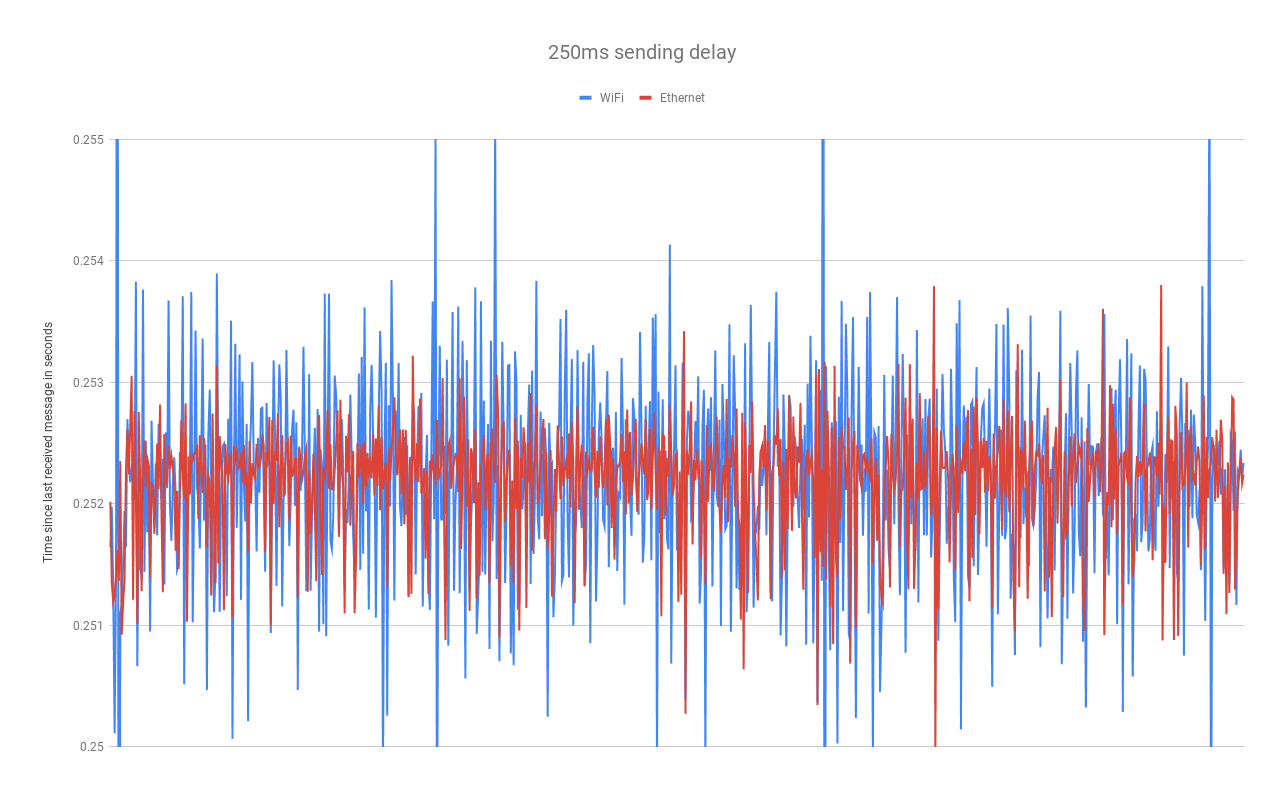
\includegraphics[width=\textwidth]{Graphs/250ms_delay}
  \caption{250ms Delay}
  \label{fig:250ms_graph}
\end{figure}

\begin{figure}[p]
  \centering
  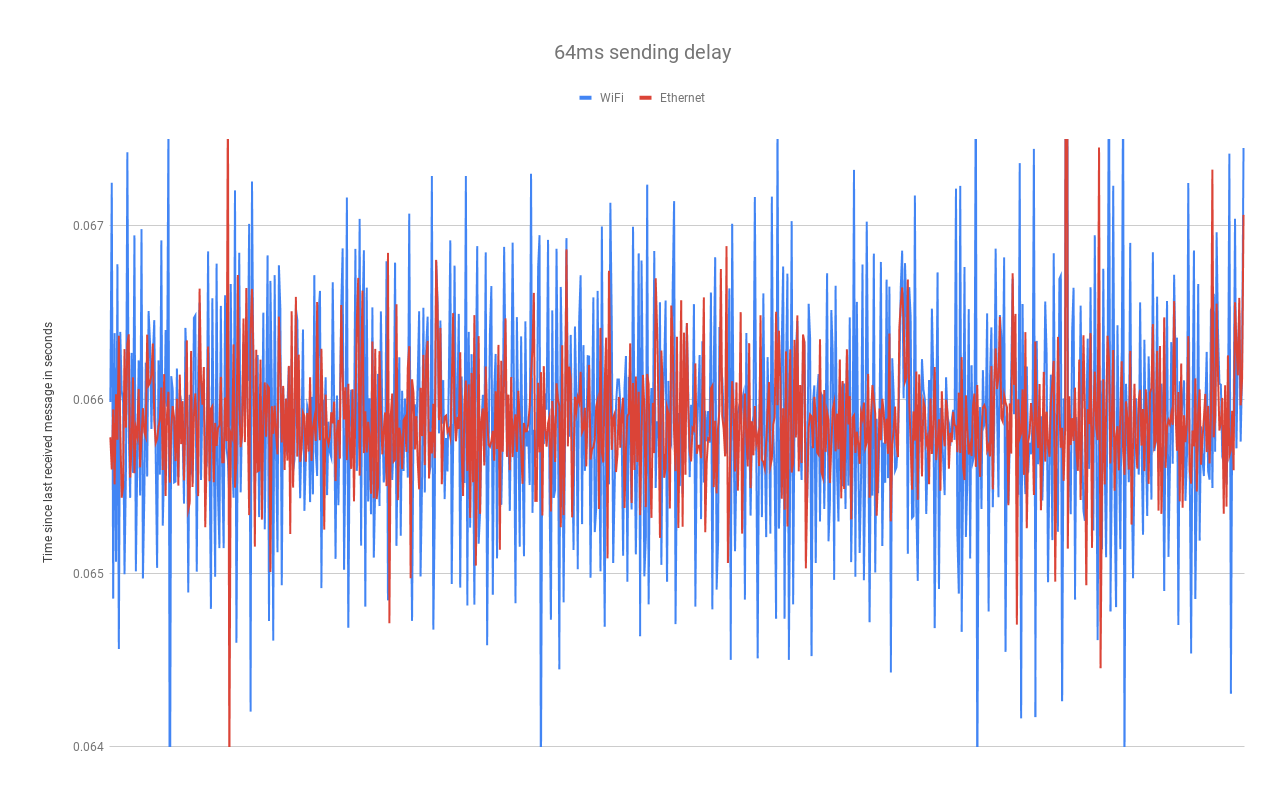
\includegraphics[width=\textwidth]{Graphs/64ms_delay}
  \caption{64ms Delay}
  \label{fig:64ms_graph}
\end{figure}

\begin{figure}[p]
  \centering
  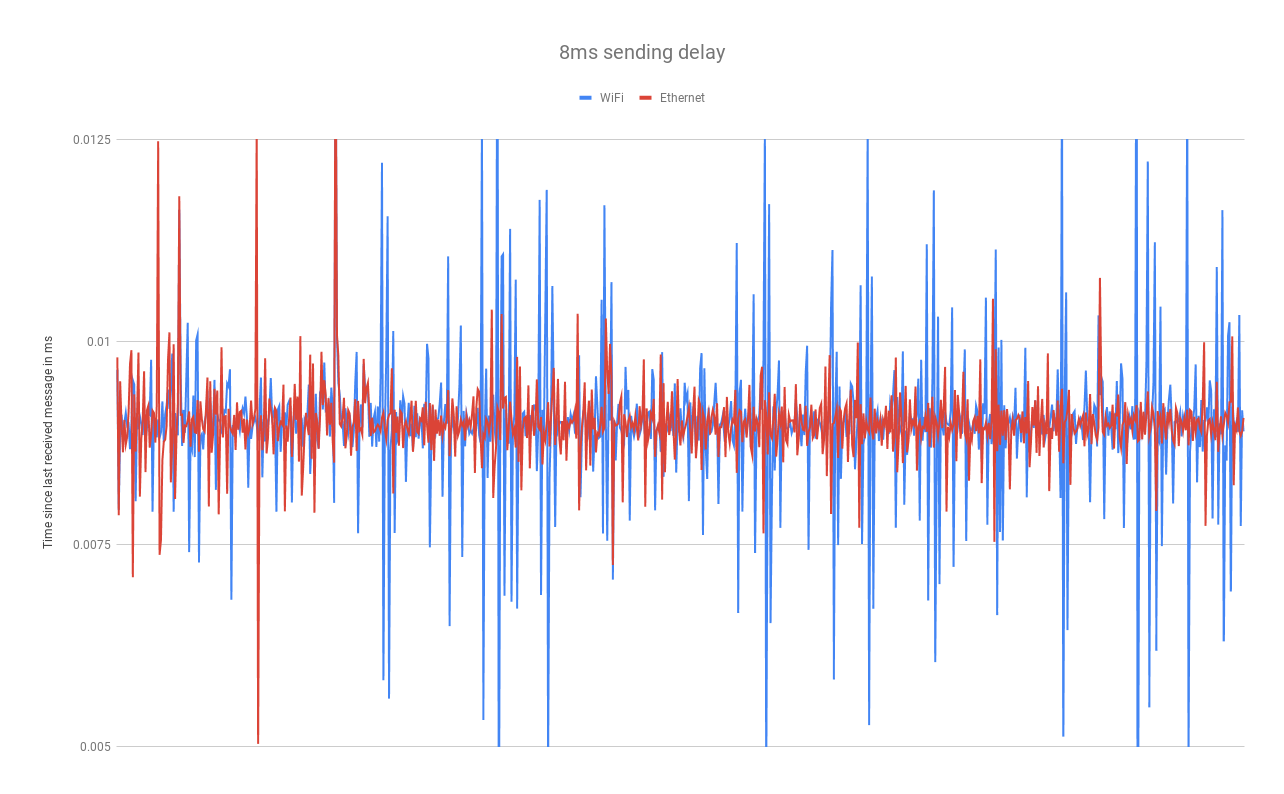
\includegraphics[width=\textwidth]{Graphs/8ms_delay}
  \caption{8ms Delay}
  \label{fig:8ms_graph}
\end{figure}



\subsection{Calculating the variance in jitter}\label{sec:variance_results}
The next question to answer was: Objectively, which collection of gathered data, had the least variance in it? This data can be seen represented in a bar chart in figure \ref{fig:jitter_variance}. The $\sigma^2$ values for WiFi at the tick-rate of 500 and 1000 milliseconds, were much larger than the other results due to having to wait for a much longer time if a packet was lost. Even when not considering these anomalous values however, it can be seen that the variance in the receiving rate is on average 30\% larger than the average of ethernet and localhost data.

One unexpected result was that even the localhost client experianced a certain level of jitter in all tests. This is likely be due to the operating system prioritising certain programs over others as well how the NIC hardware and winsock manages sending and receiving of data.

Another surprising result was once again seen at the 8ms test. Following on from the previous section, it can be seen that the variance of the data incereases when compared to the other results despite what would intuitively be the most ``reliable'' constant stream of data. The fact that the rise can be seen in all three clients, indicates that there may be some external factor (such as the host's computer's NIC or consumer grade router hardware), that interferes with these results. In general however, it is unlikely to see broadcast rates higher than 63Hz (around 16ms delay) anyway.

\begin{figure}[p]
  \centering
  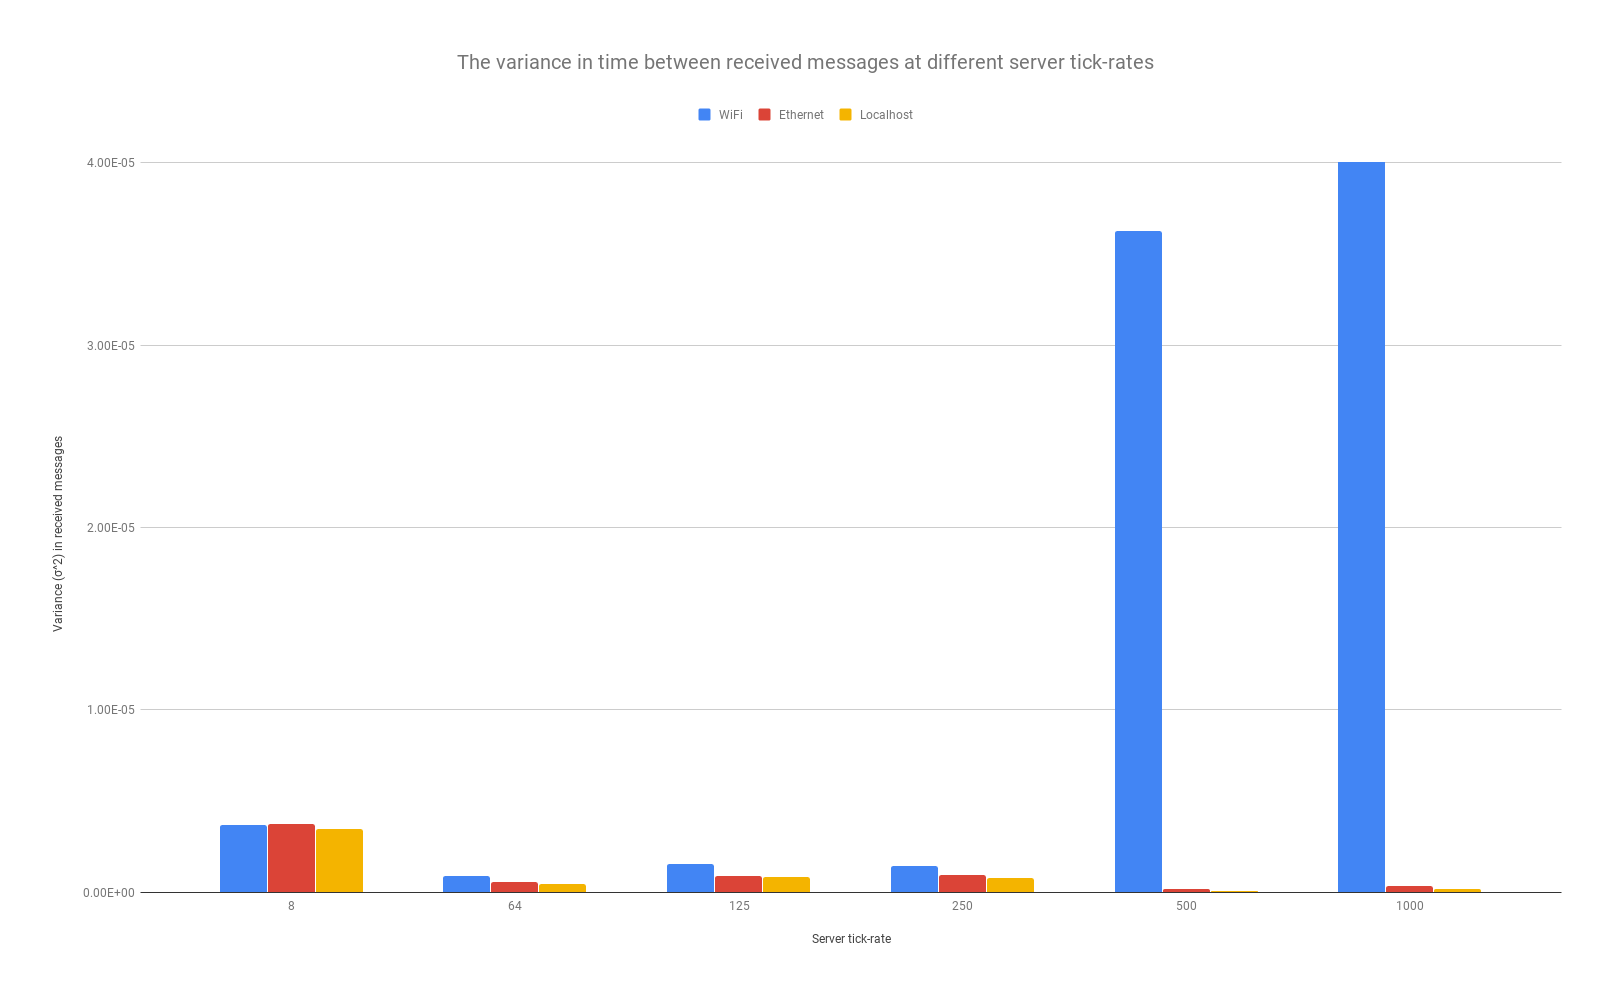
\includegraphics[width=\textwidth]{Graphs/jitter_variance}
  \caption{Graph showing the variance in the delay between receiving messages.}
  \label{fig:jitter_variance}
\end{figure}


\chapter{Conclusion}
This chapter presents a conclusion of the project based on the aims and objectives that were outlined in section \ref{sec:aims_and_objectives}. The following sections will discuss the project's success by determining if each objective has been met and as a result, if the aim of the project has been met.

\section{Satisfaction of the Aims and Objectives}
\begin{enumerate}
\item Investigate the common practices and techniques used in modern multiplayer games
  \\\\
  Extensive research into what kind of netcode different examples of popular, modern games use has been done and network development tools in the Unity game engine have been tested through real-world use. The nature of choosing a networking model is a choice that rarely has a concrete single answer. It is often the case that within the same game instance, multiple different networking models are used for synchronising different aspects of the simulation. For example, one of the players might be hosting the physics server for other players, but the rest of the simulation is synchronised through the peer to peer model, taking advantage of faster communication between any two players but having the game physics synchronised between all clients through a single instance.


\item Implement the peer to peer and client hosted networking models as a C++ library.
  \\\\
  The models' logic has been implemented into GNAT just as designed and the interface for using the current implementation is very simple.

  Below is a list of the requirements that have been outlined for the GNAT project:

  \begin{itemize}
  \item Allow for choice between the peer to peer model or the client hosted model for programs using this code.
    \\\\
    The command line application developed alongside this project uses GNAT and allows the user to choose which networking model to use.


  \item The tick rate of data broadcasting should be configurable.
    \\\\
    This has been met as the testing performed in section \ref{sec:testing}, relies on the configurable tick-rate.


  \item The only requirement to using the functionality is to clone the library in a known location. Only one import should be needed.
    \\\\
    This has been partially met. The source code successfully compiles into a static library file (GNAT\_Core.lib) however the usage of the library, differs slightly. Depending on what networking model is used, either ``peer.h'', ``client.h'' or ``server.h'' has to be included in the project. This only ends up using the necessary classes which should help with compile time on applications that use the library correctly.


  \item Every class that a user would interact with, should belong to a ``GNAT'' namespace.
    \\\\
    A user using the library has to correctly use the namespace when referring to a GNAT object. This is important as it provides code clarity if there are several object with a similar name.
\end{itemize}


\item Investigate issues spawned from computer network communication using the implemented networking models in the GNAT library.
  \\\\
  The investigation into the effect on variance that increasing the server tick-rate has, provided some insightful data.
\end{enumerate}


\section{What has been established and what could be done further}
Throughout the document, the main issues that are encountered when developing real-time, network applications, have been well established and documented. The research into the different methods of mitigating these issues have also been well researched.

Through the investigation of the modern game netcode that has been documented in the section \ref{sec:net_in_games} and beyond, it can be concluded that the most popular networking model design for games that wish to avoid a dedicated game server, is a peer to peer system with some elements of the game being moved to a client hosted server hosted by one of the peers. The state of this server is cloned periodically but the local copy is not respected and is only useful when a host migration has to occur. If a game is designed in ``zones'' that allow a player to freely enter and leave, the host migration system can be designed in such a way that as the player approaches another ``zone'', the migration process begins such that when the player fully leaves, the game does not have to pause to allow for this process to take place.

The implementation of the GNAT library has been done with minimal features and could definately be expanded further.


\section{What went well}
The investigation into netcode of popular games has proven to provide a lot of insight into the challenges that are encountered and how they can be overcome. Also, the design and implementation of the GNAT library, though not easy, has proved to be an enjoyable challenge and an invaluable learning experience.


\section{What could have been done better}
More experiments could have been performed with more varied scenarios. Some examples include:
\begin{itemize}
\item Comparing the bandwidth usage between client hosted and peer to peer models.
\item Analysis of performance of the GNAT library and how it could be made more efficient.
\end{itemize}


\section{What can be done in the future}
There are many potential improvements that could be done to build upon the foundation that have been laid out in this project through the GNAT library. Potential improvements (which have been identified in the section \ref{sec:related_work_sum}) include:
\begin{itemize}
\item It should be easier to configure the server and port address when using the library. (Ideally, the connection server configuration should be configurable during runtime)
\item The library should be easy to set up and forget. (possibly it's own thread could be started that works in the background and keeps the data synchronised).
\item It should be possible to send and receive a custom message packet at any stage in the program. (possibly a callback function could be provided that gets called whenever a given message is received)
\item Some simulation items should be synchronised automatically. (pointers to struct fields could be given to update values in the struct when a given message is received from a client.)
\end{itemize}
